Section~\ref{Sec:Reg} describes how user nodes register to become worker nodes and can be selected from the worker pool to become a producer for a ledger cycle. This section describes the work performed by producer nodes in order to maintain the ledger state. The work performed by producers in order to generate a ledger state update $\Delta L_n$ for the ledger cycle $\mathcal{C}_n$ starts at $t=t_{n,0}$ and last for a period of time $\Delta t_{cycle}$. At the end of the ledger cycle, nodes in the network use $\Delta L_n$ to update their local copy of the ledger state. This section describes the different phases of a ledger cycle. 

%%%%%%%%%%%%%%%%%%%%%%%%%%%%%%%%%%%%%

\subsection{Construction Phase}
\label{subsec:comp}

During the first phase (\textit{a.k.a} construction phase) of the ledger cycle $\mathcal{C}_n$, a producer $P_j~\forall j \in P$ creates a local ledger state update and exchanges it with its peers.\\

The first phase starts at $t = t_p = t_{n,0}$ and lasts for a period of time $\Delta t_{p}$, therefore ending at $t_p+\Delta t_{p}$.

\subsubsection{Local ledger state update generation and broadcast}

At $t = t_p$, the producer $P_j$ flushes its mempool from the $m_{n-1}$ transactions $\{Tx_i\}_{i=1,..,m_{n-1}}$ collected during the period of time [$t_{n-1,0} - \Delta t_{freeze}, t_{n,0}$] and uses these transactions to create a local ledger state update $\Delta L_{n,j}$. The production of $\Delta L_{n,j}$ lasts for a period of time [$t_p, t_p+ \Delta t_{p0}$] ($\Delta t_{c0} < \Delta t_{p}$). The producer uses a salt $s$, defined using a pseudo-random number generator that takes for seed the hash of the previous valid ledger state update $\Delta L_{n-1}$. The producer also creates a new hash tree $d_n$, to store the aggregated signature embedded in each of the $m_{n-1}$ transactions. $P_j$ then follows a series of steps: 

\begin{enumerate}
\item For each transaction $Tx_i~\forall i\in [1,m_{n-1}]$, $P_j$ verifies that the transaction is valid (see section~\ref{Sec:Val}) and if so, extracts the $n_i$ transaction entries (described in section \ref{Sec:TEnt}) $\{E_\alpha\}_{\alpha=1,...,n_i}$, included in $Tx_i$. The producer also extracts the transaction signature and adds it to the hash tree $d_n$. Note that the transactions signature in $d_n$ are sorted in alphabetic order, as to ensure that two same sets of transaction signature result in the same hash tree.

\item For each transaction entry $E_\alpha$, $P_j$ creates a corresponding hash variable: 

\begin{center}
$O_\alpha = \mathcal{H}[E_\alpha~||~s]$
\end{center}

Each pair ($E_\alpha,O_\alpha$) is added to a list $L^s_E$. Steps (1) and (2) are repeated until all transactions have been processed.

\item	$P_j$ then creates a new list $L^f_E$ using the $M=\sum_{i=1}^{m_{n-1}}n_i$ transaction entries listed in $L^s_E$ (assuming all transactions are valid) such that the transaction entries in $L^f_E = \{E_\beta\}_{\beta=1,...,M}$ are sorted following a lexicographical order based on their associated hash variable: $O_1 < O_2 < ... < O_\beta < ... < O_M$. This approach blurs the links between the token flows embedded in the transactions for a better anonymity of the users involved in said transactions.

\item $P_j$ also extracts the transaction fees $v^{f}_i$ paid in each transaction $Tx_i$ and creates the following sum:
\begin{center}
$x_f = \sum_{i=1}^{m_{n-1}} v^{f}_i$
\end{center}

\item $P_j$ computes the local ledger state update as the transactions entries list $L^f_E$ concatenated with the hash tree of the transactions signature $d_n$: 
\begin{center}
$\Delta L_{n,j} = L^f_E~||~d_n $ %+ x_f
\end{center}

The producer then computes a second quantity that represents its individual contribution:
\begin{equation}
\label{eq:hj}
\fbox{$h_j = h_{\Delta j}~||~Id_j$}
\end{equation}
with $h_{\Delta j}$ referred as the producer \textit{local hash}:
\begin{center}
$h_{\Delta j} = \mathcal{H}(\Delta L_{n,j})$ 
\end{center}
$h_j$ includes the producer unique identifier $Id_j$ (described in section \ref{Sec:PIP}), used to verify that $P_j$ is a producer node selected for the ledger cycle and later evaluate the quality of work performed by $P_j$. 

\begin{figure}[H]
\label{fig:LLSU}
\center{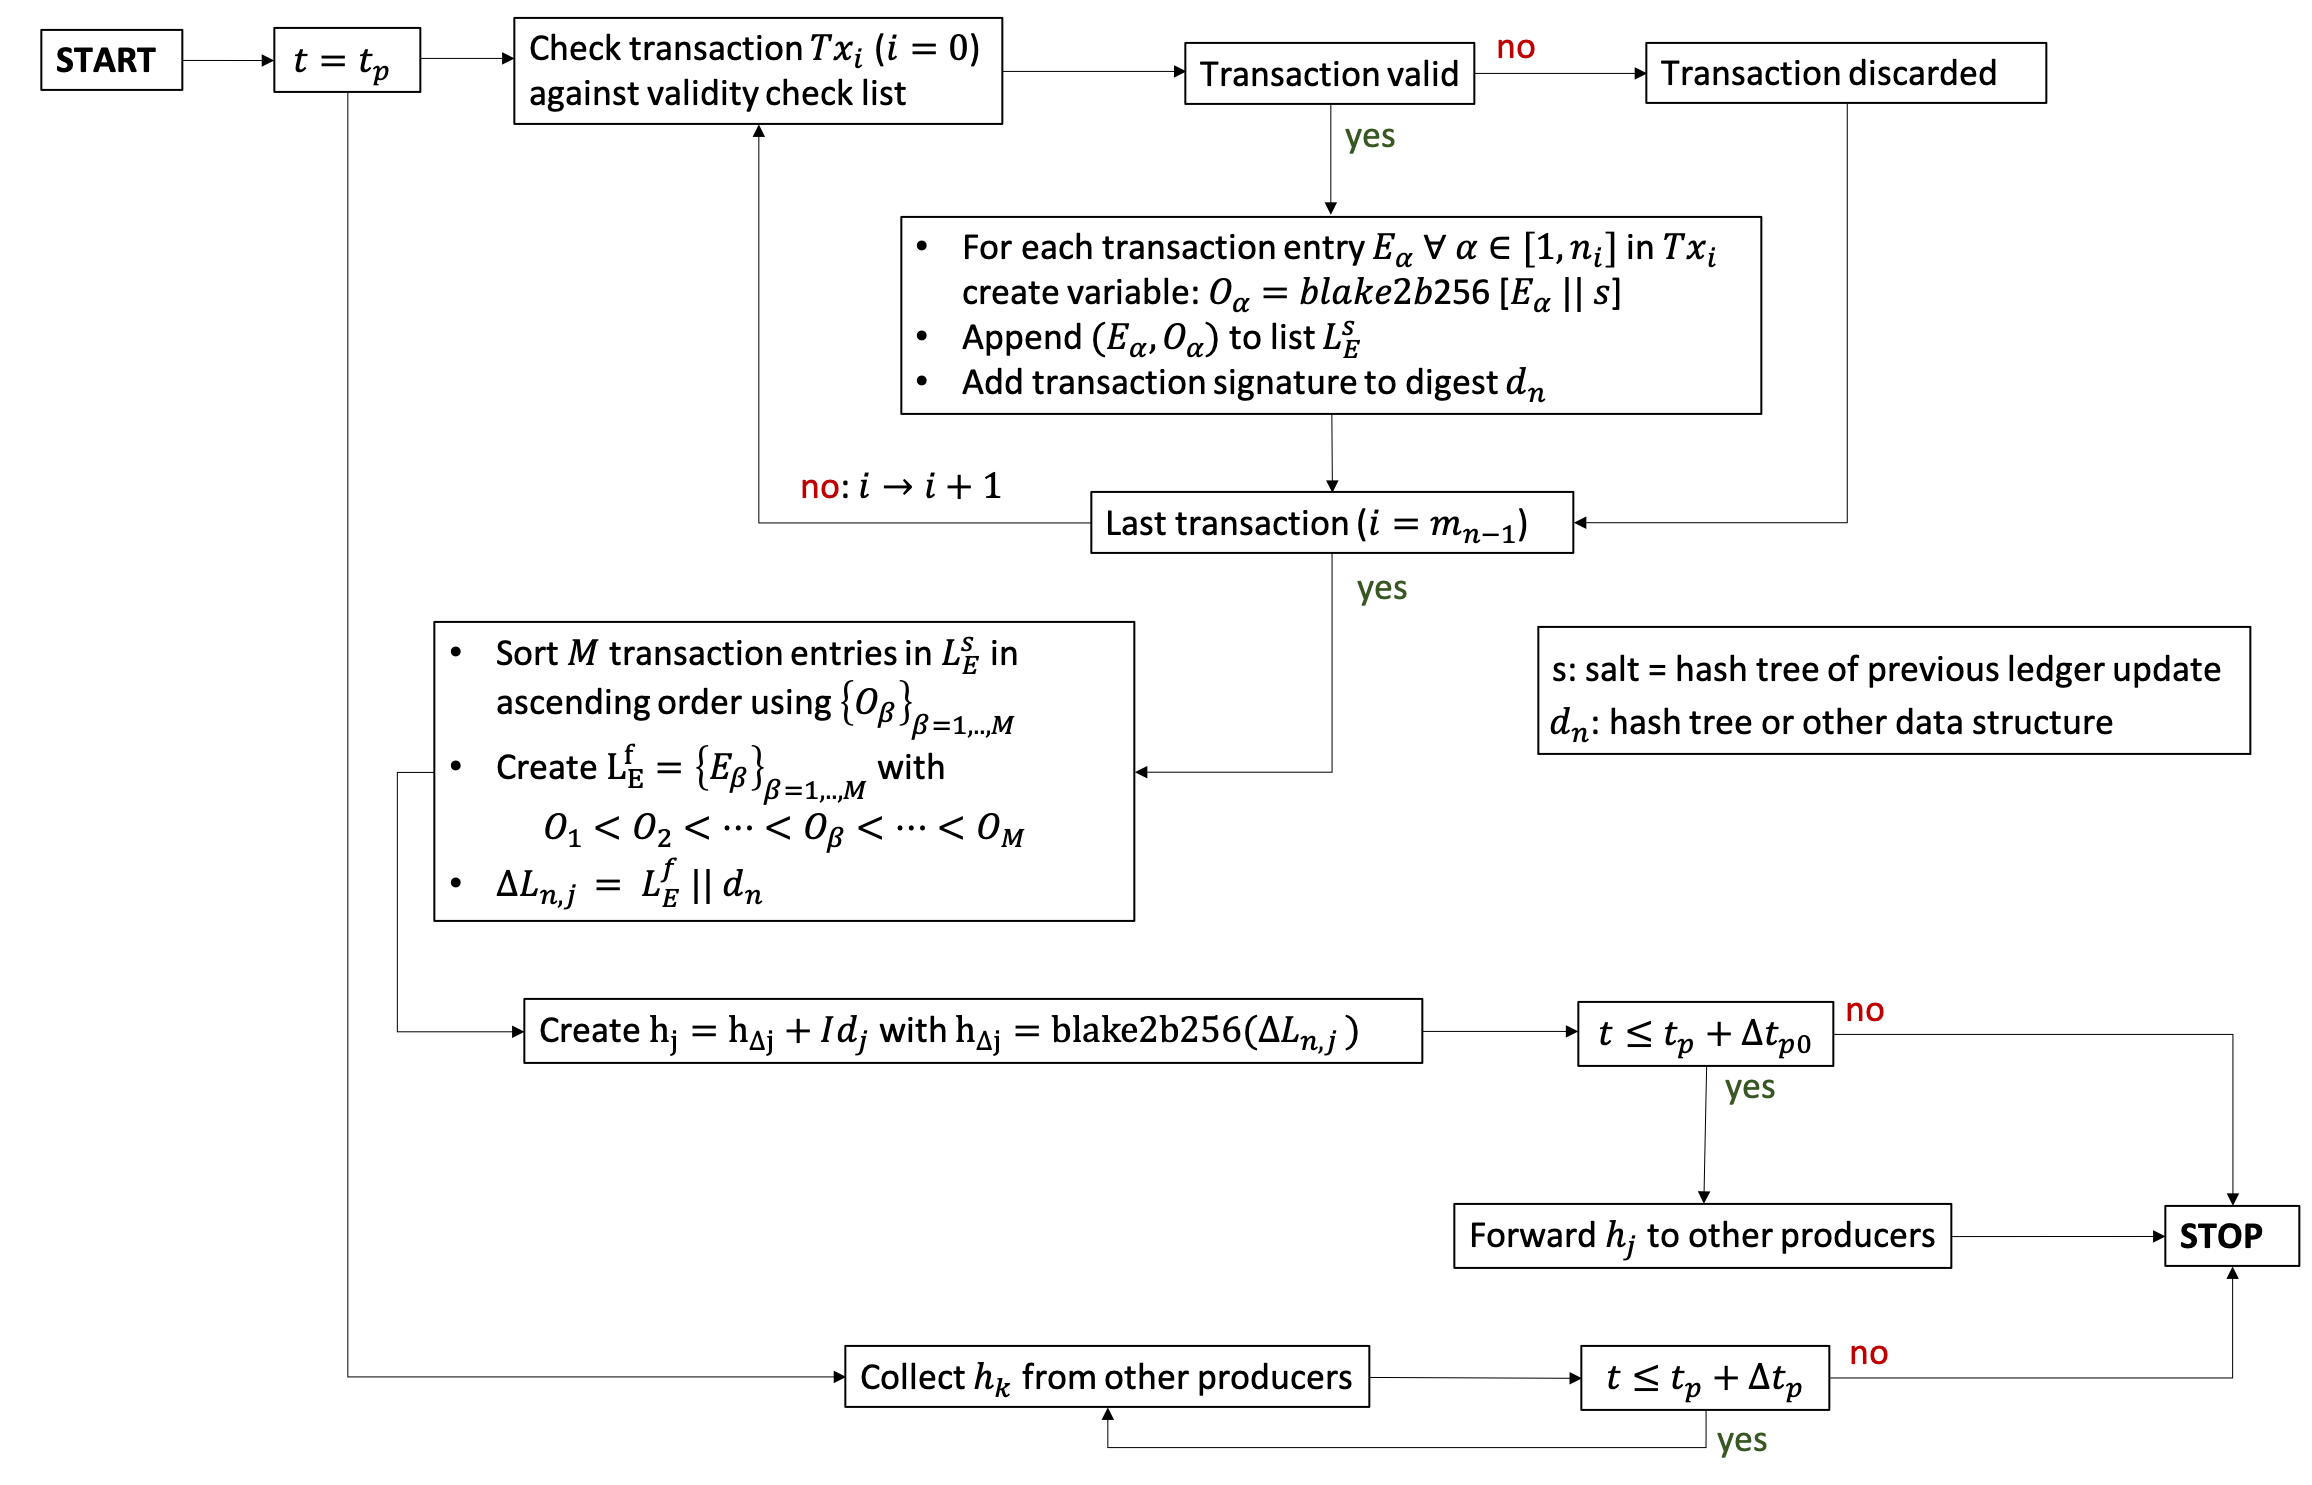
\includegraphics[width=12cm]{Figures/Local_Ledger_Computation}}
\caption{\label{fig:LLSU} Flowchart illustrated the steps followed by a producer $P_j$ node during a period of time $\Delta t_{p}$ leading to the broadcast of a local hash $h_j$.}
\end{figure}
\item At $t \leq t_p + \Delta t_{p0}$, $P_j$ broadcasts $h_j$ to the other producers in the network. Figure \ref{fig:LLSU} describes the process followed by $P_j$ to produce and broadcast $h_j$.
\end{enumerate}

\subsubsection{Local ledger state update collection}

During the first ledger cycle phase, $P_j$ collects other $\{h_k\}_{k \in P/j}$ contributions generated by its producer peers $\{P_k\}_{k \in P/j}$ in its cache. \\

At the end of the construction phase ($t = t_p + \Delta t_{p}$), $C_j$ local hashes are stored in $P_j$'s cache (including the local hash producer by $P_j$). Given the set of $P$ producers selected for the ledger cycle $\mathcal{C}_n$, the producer $P_j$ collects at most $P - 1$ contributions (\textit{e.g} $C_j = P$) with each contribution made of a local hash and a unique identifier. In an ideal world, two producers $P_j$ and $P_k$ would use the same set of transactions and as a result compute the same quantity ledger state update, leading to $\Delta L_{n,j} = \Delta L_{n,k}$. In practice, a producer may not collect exactly $P$ local hashes during $\Delta t_{p}$(\textit{e.g} $C_j \leq P$) and may not process the exact same set of transactions as its peers. The following steps describe how each producer can verify that a ledger state update has been generated by a majority of producers and generate the reward allocated to the producers. 

%%%%%%%%%%%%%%%%%%%%%%%%%%%%%%%%%%%%%

\subsection{Campaigning Phase}
\label{subsec:camp}

During the second phase (\textit{a.k.a} campaigning phase) of a ledger cycle, a producer $P_j$ designates a candidate for the correct ledger state update. At the end of the process, producers forward their proposed candidate to their peers. \\

The second phase starts at $t = t_c$ where $t_c = t_p + \Delta t_{p}$ and lasts for a period of time $\Delta t_{c}$, therefore ending at $t_c+\Delta t_{c}$.

\subsubsection{Local candidate generation and broadcast}
\label{subs:lv}
Using the $C_j$ contributions stored in its cache, $P_j$ follows a series of steps during a period of time $\Delta t_{c0}$ ($\Delta t_{c0} < \Delta t_{c}$):
\begin{enumerate}
\item $P_j$ verifies that the same local hash $h^{maj}_{\Delta j}$ is embedded in a majority $C^{maj}$ of contributions, where $h^{maj}_{\Delta j}= max[unique(h_{\Delta k})~\forall~k\in\{C_j\}]$ and $C^{maj} = count[(h_{\Delta k} = h^{maj}_{\Delta j})~\forall~k\in\{C_j\}]$. The threshold, $C_{threshold}$, to decide if a majority of producers agrees on the same ledger state update, should be strictly greater than 50\%, due to statistical consideration. The relevant variables for a producer to decide if the same ledger state update is found by a majority of producers are $C_{min}$ and $C^{maj}$. Threshold considerations are discussed in detail in section~\ref{Sec:SecLsu}. 

If $C_j > C_{min}$ and $C^{maj} > C_{threshold}$ :

\begin{itemize}
\item $P_j$ creates a list $\mathcal{L}_j(prod)$ and appends to said list the identifiers of any producer $P_k$ who forwarded a contribution $h_k$ satisfying $h_{\Delta k} = h^{maj}_{\Delta j}$.\\
If $h_{\Delta j}= h^{maj}_{\Delta j}$, $P_j$ also appends its identifier to the list $\mathcal{L}_j(prod)$.
\item The producer $P_j$ then computes the following quantity: 

\begin{equation}
\label{eq:cj}
\fbox{$c_j = h^{maj}_{\Delta j}~||~\#(L_j(prod))~||~Id_j$}
\end{equation}

Where \# represents a hash tree or some other compressed data structure of the list $L_j(prod)$. $c_j$ corresponds to $P_j$'s candidate for the most popular ledger state update. A hash tree of a list is useful to quickly verify that an object (an identifier) is included in the list. $\#(\mathcal{L}_j(prod))$ is a witness of the list of producers who correctly generated the most popular ledger state update according to $P_j$. 
\item At $t \leq t_c+\Delta t_{c0}$, $P_j$ broadcasts its candidate $c_j$ to the other producers in the network. Figure \ref{fig:computation} displays a flowchart describing the steps followed by $P_j$ to create and broadcast $c_j$.
\end{itemize}

\begin{figure}[H]
\label{fig:computation}
\center{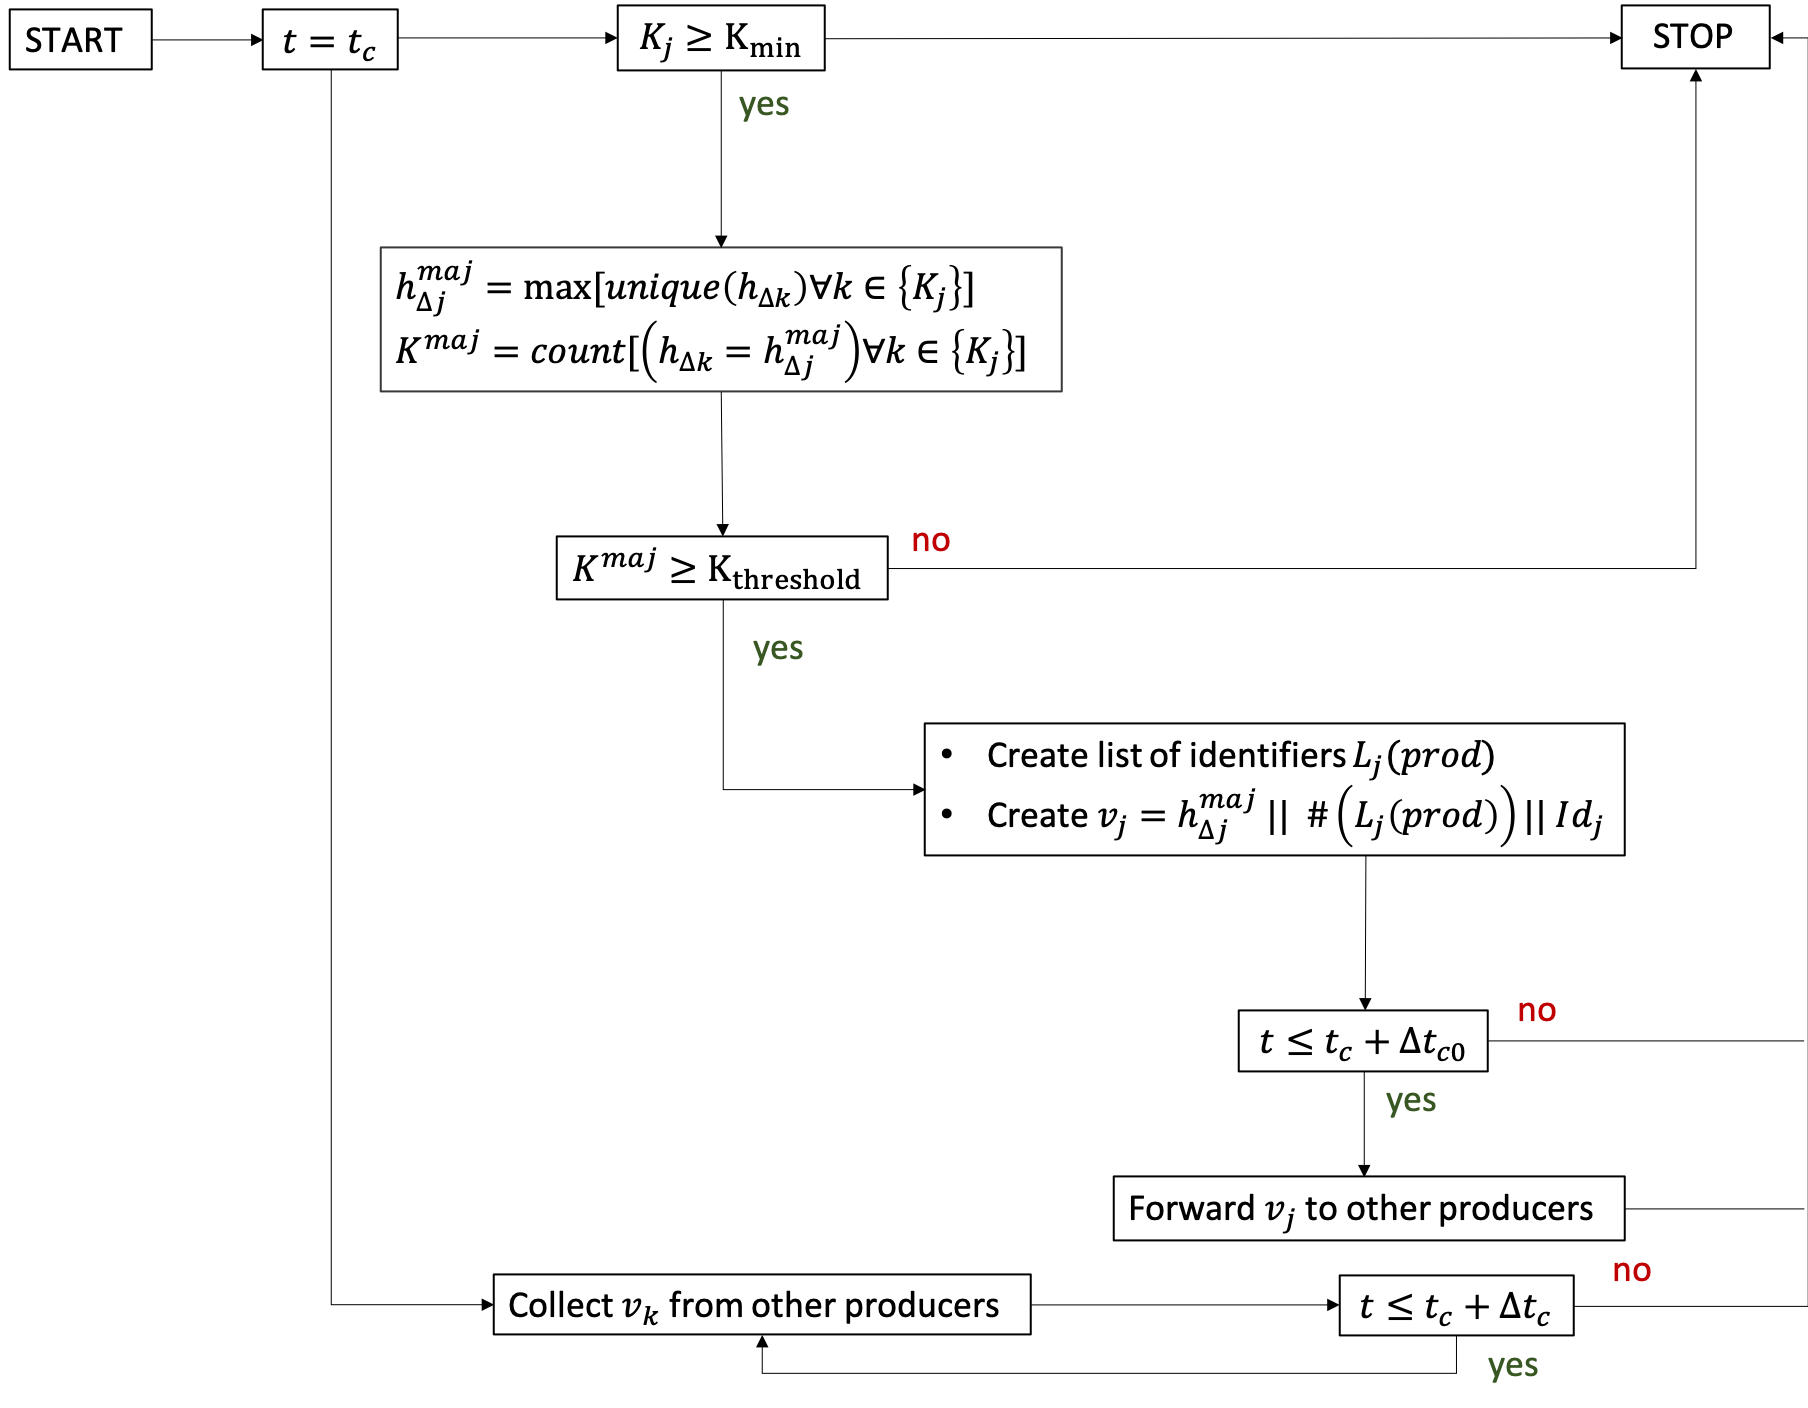
\includegraphics[width=12cm]{Figures/Local_Vote_Broadcast}}
\caption{\label{fig:computation} Flowchart illustrating the series of steps followed by a producer $P_j$ to issue a candidate $c_j$.}
\end{figure}
\end{enumerate}

\subsubsection{Local candidate collection}
Shortly after the second phase starts (at $t \approx t_c$), $P_j$ starts collecting other candidates $c_{k}$ generated by other producers $\{P_k\}_{k \in P/j}$ in its cache. The collection lasts for a period of time $\Delta t_{c}$ after which the producer holds $V_j$ candidates in its cache ($V_{min} \leq V_j \leq P$). 

\subsection{Voting Phase}
\label{subsec:vote}

During the third phase (\textit{a.k.a} voting phase) of a ledger cycle, a producer $P_j$ votes on the correct ledger state update. At the end of the process, producers forward their proposed ledger state update including a reward to some producers to their peers. \\

The third phase starts at $t = t_v$ where $t_v = t_p + \Delta t_{p} + \Delta t_{c}$ and lasts for a period of time $\Delta t_{v}$, therefore ending at $t_v+\Delta t_{v}$.


\subsubsection{Ballot generation and broadcast}
At $t = t_v$:
\begin{enumerate}
\item $P_j$ verifies that the same local hash $h^{maj}$ is embedded in a majority of candidates. With $h^{maj} = max[unique(h^{maj}_{\Delta k})~\forall~k\in\{V_j\}]$ and $V^{maj} = count[(h^{maj}_{\Delta k} = h^{maj})~\forall~k\in\{V_j\}]$, this condition is met if $V^{maj} > V_{threshold}$ (See section~\ref{Sec:SecLsu} for more explanations). 
\item The producer $P_j$ can only participate in the following steps if the local hash computed during the computation phase, $h_{\Delta j}$, is equal to $h^{maj}$. Indeed, $P_j$ needs to have knowledge of the ledger state update of which the hash was used to vote in order to proceed. 
\end{enumerate}
 
If each producer collects the local hash generated by every producer, any two producers $P_j$ and $P_k$ would build the same list of identifiers $\mathcal{L}_j(prod) = \mathcal{L}_k(prod)$. In practice, a producer may not have collected all local hashes and as a result have an incomplete list of identifiers, yet have collected enough data to be able to issue a correct vote. We mentioned how the identifier of a producer can be appended to a local hash to verify that $P_j$ is a producer node selected for the ledger cycle and evaluate the quality of work performed by $P_j$. Indeed, $Id_j$ can be used to create and add a compensation entry to the ledger state update, that rewards the producer for its work performed during the ledger cycle. The correct (complete) list of producers who successfully built the correct (dominant) ledger state update for that cycle, $\mathcal{L}_n(prod)$, is used to create these new transaction entries and append them to the final ledger state update generated for that cycle. It is therefore crucial that a majority of producers succeed in generating that list in order to generate the same final ledger state update. \\ 


The voting process thus consists in creating the final list of identifiers involved in the production of the ledger state update. As explained below the final list $\mathcal{L}_n(prod)$ is obtained by merging the partial lists included in the producers' vote. A producer $P_j$ could have produced a different hash $h_{\Delta j}$ to $h^{maj}_{\Delta j}$ yet added his identifier to $\mathcal{L}_j(prod)$ in the attempt to get some token reward allocated to producers who correctly produced the next ledger state update. In such scenario $Id_j$ would be an element of the list included in $c_j$ (or any other producer node controlled by $P_j$), but it wouldn't be included in any other list $\{\mathcal{L}_k(prod)\} \forall~k \in P/j\}$. To prevent such malicious behaviour, a rule imposes that $P_j$ only append to the final list $\mathcal{L}_n(prod)$ the identifier of a producer included in the list $\mathcal{L}_k(prod)$ of a candidate $c_k$ satisfying $h^{maj}_{\Delta k} = h^{maj}$ if and only if that identifier is included in at least $P/2$ lists $\{\mathcal{L}_{k}(prod)\}_{k=1,..,V_j}$ associated to a candidate $c_{k}$ satisfying $h^{maj}_{\Delta k} = h^{maj}$. Although this eliminates the risk of unethical behaviour from the producer, this also means that there would be little incentive for a producer to broadcast its vote if its identifier was not included in $\mathcal{L}_n(prod)$. However, the probability that a producer compiles the correct final list $\mathcal{L}_n(prod)$ strongly depends on the number of votes collected. The more votes collected by a producer, the greater the probability that said producer will compile the complete final list. Although a producer may not have produced the correct local ledger state update, participating in the voting process is, therefore, an important contribution to the overall consensus protocol and should entitle the producer to some reward. To that end a producer $P_j$ can use the identifier of other producers included in their vote and create a second list $\mathcal{L}_j(vote)$ to account for their participation in the voting process. \\
 
$P_j$ follows a series of step for a period of time $\Delta t_{v0}$ ($\Delta t_{v0} < \Delta t_{v}$):

\begin{enumerate}
\item $P_j$ creates a new list $\mathcal{L}_j(vote)$ and appends to said list the identifier of any producer $P_k$ who forwarded a candidate $c_k$ satisfying $h^{maj}_{\Delta k} = h^{maj}$.
\item $P_j$ creates the final list $\mathcal{L}_n(prod)$ and appends to said list the identifier of a producer included in the list $\mathcal{L}_k(prod)$ of a candidate $c_k$ satisfying $h^{maj}_{\Delta k} = h^{maj}$ if and only if that identifier is included in at least $P/2$ lists $\{\mathcal{L}_{k}(prod)\}_{k=1,..,V_j}$ associated to a candidate $c_{k}$ satisfying $h^{maj}_{\Delta k} = h^{maj}$. 
\item $P_j$ then creates a list $L_{CE}$ of compensation entries for each producer whose identifier is included in $\mathcal{L}_n(prod)$. Each producer receives $x_h$ tokens. Assume that $ C_n \leq P$ identifiers are included in $\mathcal{L}_n(prod)$ and $X$ is the total number of tokens injected per cycle for the pool of $P$ producers. The quantity $x_h$ is defined such that $ C_nx_h = f_{prod}X + x_f$ where $x_f$ represents the total number of fees collected from the $m_{n-1}$ transactions and $f_{prod}$ represents the fraction of new tokens injected per cycle and distributed to the producers who built the correct ledger state update. The remaining $(1-f_{prod})X$ tokens are distributed to other contributing nodes in the network. A part of this remainder goes to the producers who voted correctly on the previous ledger cycle update. Let $\mathcal{L}_{n-1}(vote)$ be the list of the identifiers of producers who voted correctly on the previous ledger cycle update $\mathcal{C}_{n-1}$. We later demonstrate how such a list is derived during a ledger cycle. For now, let's assume that $L_{CE}$ includes compensation entries for producers involved the production of the ledger state update for this ledger cycle $\mathcal{C}_n$ and the producers involved in the voting process of the precedent cycle $\mathcal{C}_{n-1}$. 
\item $P_j$ then creates the final ledger state update for $\mathcal{C}_n$ including the reward allocated to the producers for their contribution:
\begin{center}
$\mathbf{LSU_j = L^f_E~||~d_n~||~L_{CE}}$
\end{center}
$P_j$ then computes its final vote (or ballot):
\begin{equation}
\label{eq:vj}
\fbox{$v_j = \mathcal{H}(LSU_j)~||~\#(\mathcal{L}_j(vote))~||~Id_j$}
\end{equation}

which includes a partial list of identifiers of producers who designated the correct candidate for the ledger state update $h^{maj}$. 

\item $P_j$ then forwards $v_j$ to the other producers and collect the votes issued by its peers. Figure \ref{fig:Vot} illustrates the different steps followed by $P_j$ during the voting phase.
\begin{figure}[H]
\label{fig:Vot}
\center{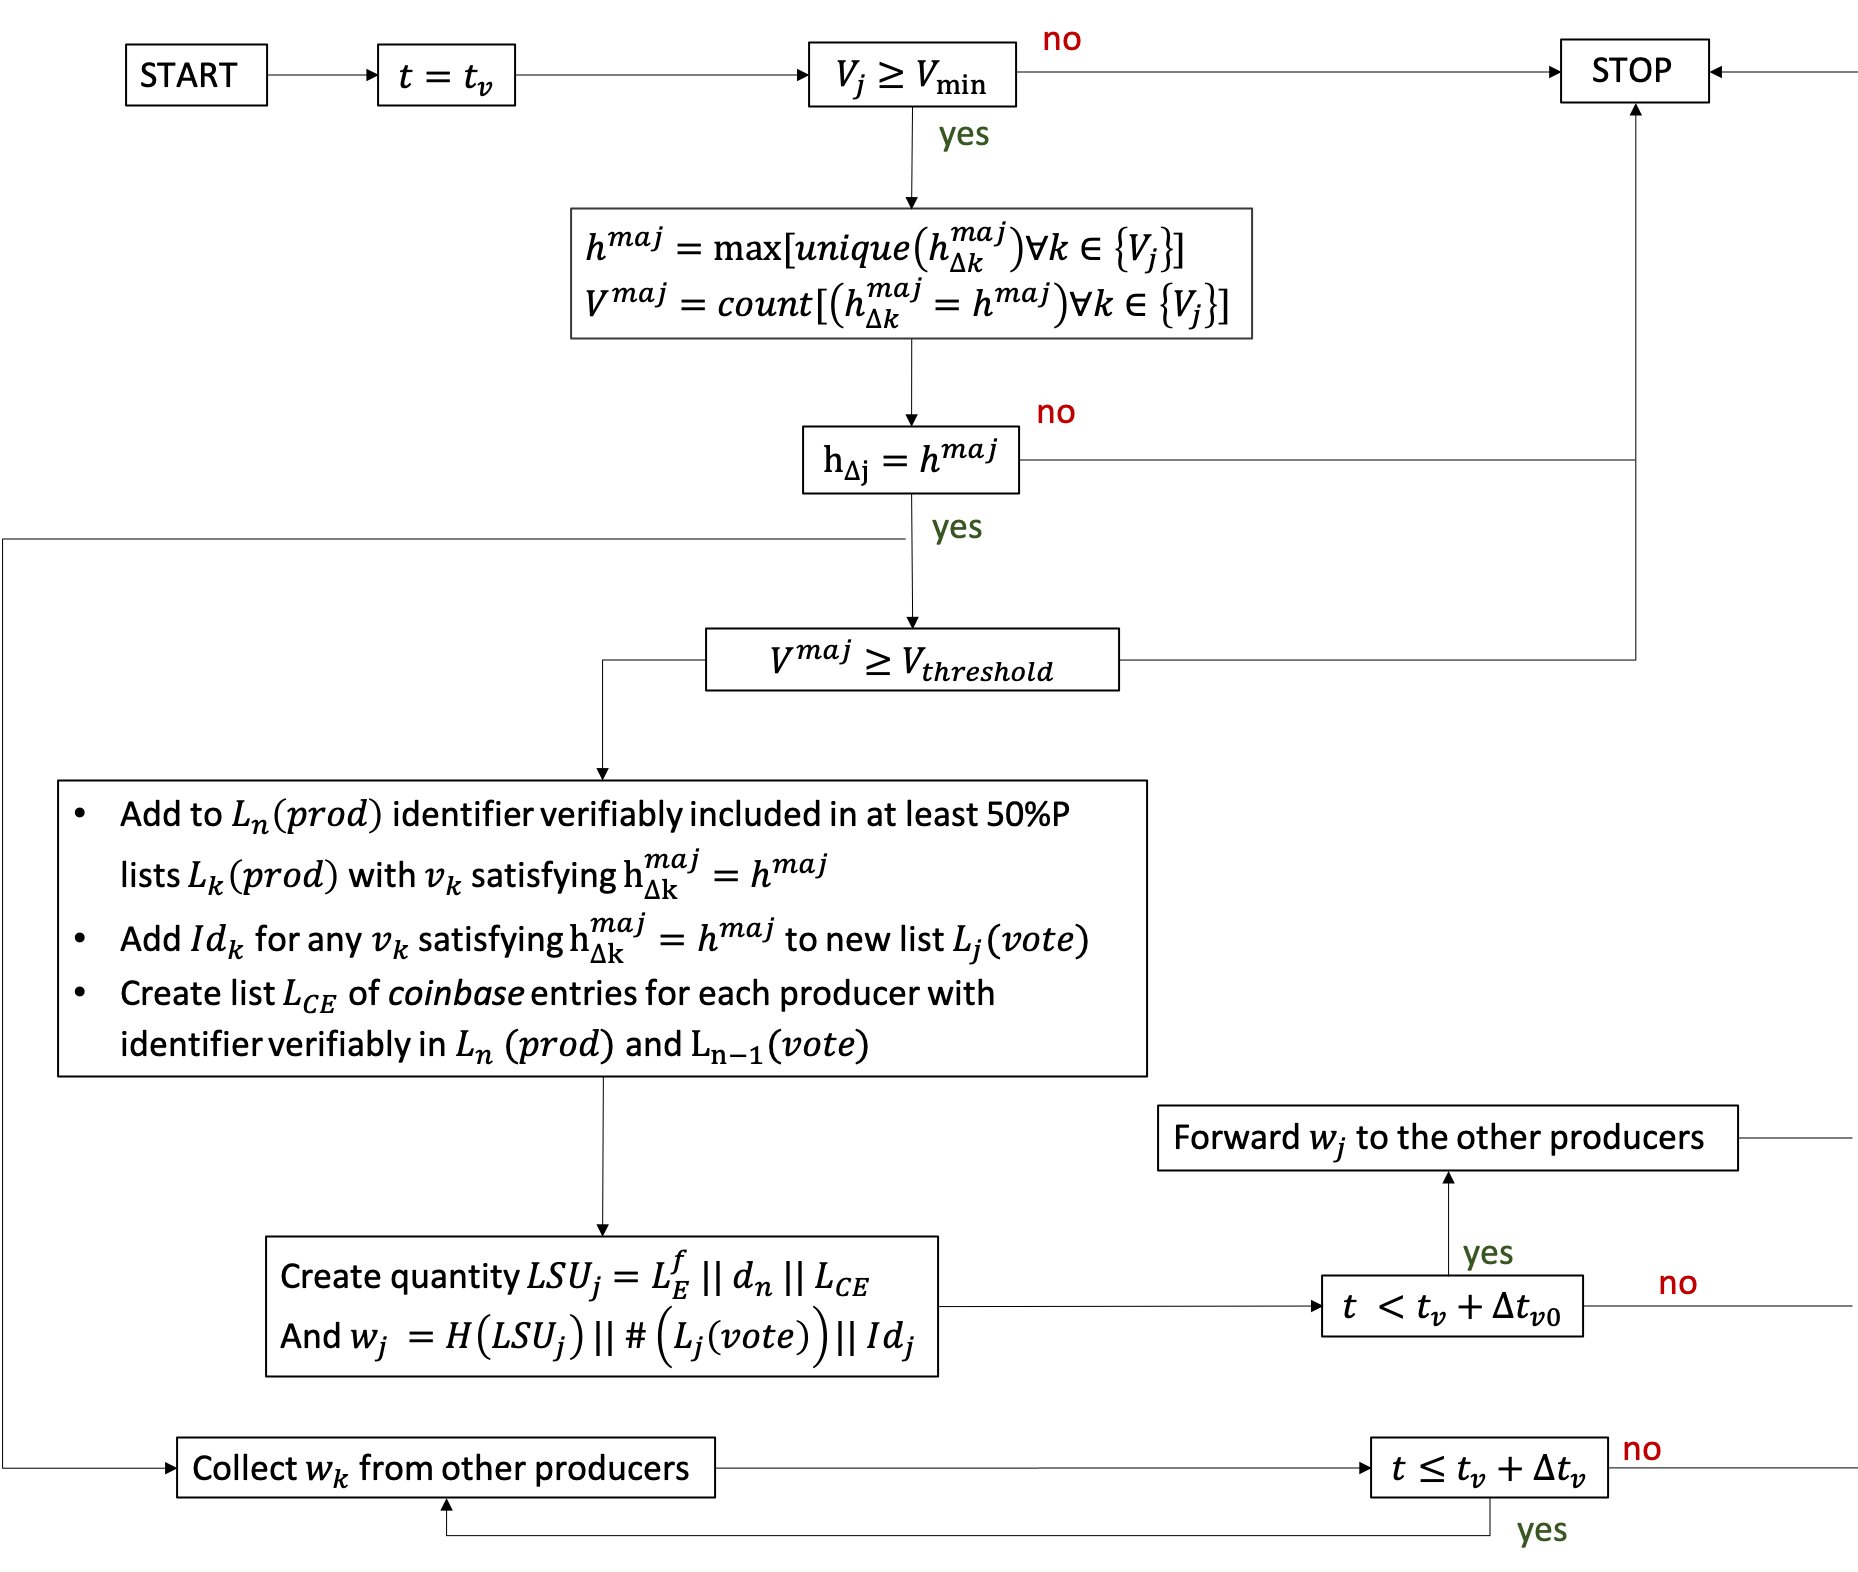
\includegraphics[width=11cm]{Figures/Global_Vote_Broadcast}}
\caption{\label{fig:Vot}Flowchart illustrating the series of steps followed by a producer $P_j$ during the voting phase of the ledger cycle.}
\end{figure}
\end{enumerate}


\subsubsection{Ballot collection}
During the voting phase, the producer $P_j$ collects the votes broadcast by its peers. At the end of the voting phase ($t = t_v+\Delta t_{v}$), the producer $P_j$ holds $U_j$ final votes in its cache with $U_j \leq C_n$ where $C_n \leq P$ is the actual total number of producers who correctly computed $h^{maj}$.

%%%%%%%%%%%%%%%%%%%%%%%%%%%%%%%%%%%%%

\subsection{Synchronisation Phase}
\label{subsec:sync}
\subsubsection{Final ledger state update generation and broadcast}

The last phase (\textit{a.k.a} synchronisation phase) of a ledger cycle starts at $t = t_s$, with $t_s = t_{n,0} + \Delta t_{p} + \Delta t_{c}+ \Delta t_{v}$, and lasts for a period of time $\Delta t_{s}$, therefore ending at $t_s+\Delta t_s = t_{n,0} + \Delta t_{cycle}$.

During a period of time $\Delta t_{s0} < \Delta t_{s}$, $P_j$ executes the following steps:

\begin{enumerate}
\item $P_j$ defines the ledger state update $\Delta L_n$ for the cycle $\mathcal{C}_n$ as:\\
 $\mathcal{H}(\Delta L_n) = max[unique(\mathcal{H}(LSU_k))~\forall~k\in\{U_j\}]$ and the associated number of votes collected: $U^{maj} = count[(\mathcal{H}(LSU_k) = \mathcal{H}(\Delta L_n))~\forall~k\in\{U_j\}]$ and verifies that $U^{maj}> U_{threshold}$.
\item $P_j$ creates a new list $\mathcal{L}_{n}(vote)$ and appends to $\mathcal{L}_{n}(vote)$ the identifier of a producer included in the list $\mathcal{L}_{k}(vote)$ of a vote $v_k$ satisfying $\mathcal{H}(LSU_k) = \mathcal{H}(\Delta L_n)$ if and only if the identifier is included in at least $C_n/2$ lists $\{\mathcal{L}_{k}(vote)\}$ associated to a vote $v_{k}$ satisfying $\mathcal{H}(LSU_k) = \mathcal{H}(\Delta L_n)$. Note that $C_n$ can be easily computed as it corresponds to the number of producer identifiers who correctly computed the ledger state update and are therefore included in $\mathcal{L}_{n}(prod)$.
\begin{comment}
\item $P_j$ then creates the following quantities:
\begin{equation} 
\fbox{$\mathbf{H_{j} = \mathcal{H}(\Delta L_n)~||~\#(\mathcal{L}_{n}(vote))~||~Id_j}$}
\label{eq:Hj}
\end{equation}
\end{comment}
\item If $P_j$ generated the correct ledger state update $\Delta L_n$, it can write it to DFS which will return it with a content based address $\mathcal{A}_n$. 
\item A Producer $P_j$ then creates the following quantity:
\begin{equation} 
\fbox{$\mathbf{H_{j} = \mathcal{A}_n~||~\#(\mathcal{L}_{n}(vote))~||~Id_j}$}
\label{eq:Hj}
\end{equation}
The producer then broadcasts $H_j$ to the network.% Worker nodes, as well as DFS nodes collect the quantities $\{H_k\}_{\forall~k\in\{P\}}$. %Upon receiving individuals quantities, workers store $\#(\mathcal{L}_{n}(vote))$ in their mempool. 
\end{enumerate}


\subsubsection{Ledger state synchronisation across the network}

During the time period [$t_{s}, t_s + \Delta t_{cycle}$], user nodes collect $\{H_k\}_{\forall k \in P}$ quantities broadcast by the producers. 
By extracting the identifier $Id_k$ embedded in any collected quantity $H_k$, a user node can easily compile a list of producer identifiers having broadcast the same quantity $\mathcal{H}(\Delta L_n)$ (concatenated with the same list $\mathcal{L}_{n}(vote)$). Upon receiving $x > P/2$ identical addresses $\{\mathcal{A}_k = \mathcal{A}_n\}_{k \in x}$, the user nodes can read the common address content ($\Delta L_n$) from DFS. Using $\Delta L_n$ a user node can safely synchronise their local copy of the ledger and write it to their DFS if not already done. The balance of accounts stored on the ledger are updated and the producers effectively collect their rewards.\\


Worker nodes also store the list $\mathcal{L}_{n}(vote)$ embedded in each $H_k$ quantity. If selected to be a producer for the next cycle $\mathcal{C}_{n+1}$, a worker can use it to generate the reward allocated to the producers who correctly voted for the accurate ledger state update during the ledger cycle $\mathcal{C}_{n}$.\\


\begin{comment}
Producers having generated the correct ledger state update $\Delta L_n$ can write it to DFS. 


During the time period [$t_{s}, t_s + \Delta t_{cycle}$], worker nodes, as well as DFS nodes collect $\{H_k\}_{\forall k \in P}$ quantities broadcast by the producers. 
By extracting the identifier $Id_k$ embedded in any collected quantity $H_k$, a DFS node can easily compile a list of producer identifiers having broadcast the same quantity $\mathcal{H}(\Delta L_n)$ (concatenated with the same list $\mathcal{L}_{n}(vote)$). Producers having generated the correct ledger state update $\Delta L_n$ can forward it to DFS nodes.
User nodes can collect the  content based address from producer nodes. 

The nodes which have the correct delta can all write it to the DFS. It will return them with a content based address, which is a sort of hash. Then if you dont have the hash (because you didn't have the content) you can collect it from a majority x > P/2 and read its content from the DFS. That is my understading.
Once a DFS node has collected $x \geq P/2$ identical hash values, they can accept any $\Delta L_n$ value matching $\mathcal{H}(\Delta L_n)$. User nodes can then request the ledger state update $\Delta L_n$ from DFS nodes and safely synchronise their local copy to the ledger. The balance of accounts stored on the ledger are updated and the producers effectively collect their rewards. \\

\end{comment}

Figure~\ref{fig:cycle} summarises the different phases of the ledger cycle.\\

The various parameters and thresholds mentioned in this chapter and their impact on the levels of security and confidence in the successful production of a ledger state update are discussed in section~\ref{Sec:SecLsu}.
\newpage
\begin{landscape}
\begin{figure}
\center
    \includegraphics[width=22cm,height=42cm,keepaspectratio]{Figures/Catalyst_cycle}
    \caption{\label{fig:cycle}Illustration of the different phases followed by a producer during a ledger cycle.}
\end{figure}
\end{landscape}

